\documentclass[10pt, aspectratio=169]{beamer}
\usefonttheme{professionalfonts}

\mode<presentation>
{
  \usetheme{Berkeley}
  \usecolortheme{beaver}
  \usefonttheme{default}
  \setbeamertemplate{navigation symbols}{}
  \setbeamertemplate{caption}[numbered]
} 

\setbeamertemplate{footline}{%
  \leavevmode%
  \hbox{%
    \begin{beamercolorbox}[wd=.85\paperwidth,ht=2.5ex,dp=1ex,left]{author in head/foot}%
      \usebeamerfont{author in head/foot}Maxx Seminario, Electronic Circuits, Spring 2026%
    \end{beamercolorbox}%
    \begin{beamercolorbox}[wd=.15\paperwidth,ht=2.5ex,dp=1ex,right]{date in head/foot}%
      \hspace*{0.5em}\insertframenumber{} / \inserttotalframenumber\hspace*{0.5em}%
    \end{beamercolorbox}%
  }%
  \vskip0pt%
}

\usepackage[english]{babel}
\usepackage[utf8x]{inputenc}
\usepackage{tikz}
\usetikzlibrary{shapes.geometric}
\usepackage{pgfplots}
\usepackage{array}
\usepackage{makecell}
\usepackage{verbatim}
\usepackage{graphicx}
\usepackage{subcaption}
\usepackage{amsfonts}
\usepackage{amsmath}
\usepackage{bm}
\usepackage{epstopdf}
\usepackage{circuitikz}
\usepackage{caption}
\usepackage{multirow}
\captionsetup{compatibility=false}
\usepackage[absolute,overlay]{textpos}
\usetikzlibrary{calc}
\usetikzlibrary{pgfplots.fillbetween, backgrounds}
\usetikzlibrary{positioning}
\usetikzlibrary{pgfplots.groupplots}
\usetikzlibrary{plotmarks}
\usetikzlibrary{calc}

\pgfplotsset{compat=1.16}

% Added by Maxx Seminario 01/06/2026 - for colored icons in itemize labels
\usepackage{wasysym} % for smiles and frowns
\newcommand{\neutralface}{%
  \tikz[baseline=-0.6ex]{
    \draw (0,0) circle (0.9ex);
    \fill (-0.35ex,0.25ex) circle (0.12ex);
    \fill ( 0.35ex,0.25ex) circle (0.12ex);
    \draw (-0.35ex,-0.25ex) -- (0.35ex,-0.25ex);
  }%
}

\newcommand{\baditem}{\textcolor{red!70!black}{\frownie}}
\newcommand{\gooditem}{\textcolor{green!60!black}{\smiley}}
\newcommand{\mehitem}{\textcolor{orange!80!black}{\neutralface}}


% =========================
% Solution toggle 
% =========================
\newif\ifshowsolutions
\showsolutionstrue   %  compile WITH solutions
%\showsolutionsfalse %  compile WITHOUT solutions



\title{MOSFET AC Analysis and Small-Signal Models}
\subtitle{Unit 5: Field-Effect Transistors}
\author{Maxx Seminario}
\institute{University of Nebraska-Lincoln}
\date{Spring 2026}

\begin{document}

\begin{frame}
  \titlepage
\end{frame}

% % Slide 2: Lecture Overview
% \begin{frame}{Lecture Overview}
% \begin{columns}[T]
% \begin{column}{0.45\textwidth}
% \textbf{Review from Last Lecture}
% \begin{itemize}
% \item MOSFET DC biasing techniques
% \item Q-point determination
% \item DC operating regions
% \item Bias circuit design
% \end{itemize}
% \end{column}

% \begin{column}{0.45\textwidth}
% \textbf{Learning Objectives}
% \begin{itemize}
% \item Derive MOSFET small-signal model
% \item Analyze AC behavior including field effect
% \item Incorporate channel-length modulation (CLM)
% \item Calculate small-signal parameters ($g_m$, $r_o$)
% \end{itemize}
% \end{column}
% \end{columns}
% \end{frame}

% Slide 3: AC vs DC Analysis
\begin{frame}{AC vs DC Analysis}
\begin{columns}
\begin{column}{0.5\textwidth}
\textbf{DC Analysis}
\begin{itemize}
\item Establishes Q-point
\item Determines operating region
\item Uses large-signal model
\item Static voltages and currents
\end{itemize}

\vspace{0.5cm}
\textbf{AC Analysis}
\begin{itemize}
\item Small variations around Q-point
\item Uses small-signal model
\item Linear approximation
\item Frequency-dependent behavior
\end{itemize}
\end{column}

\begin{column}{0.5\textwidth}
\textbf{Total Signal = DC + AC}

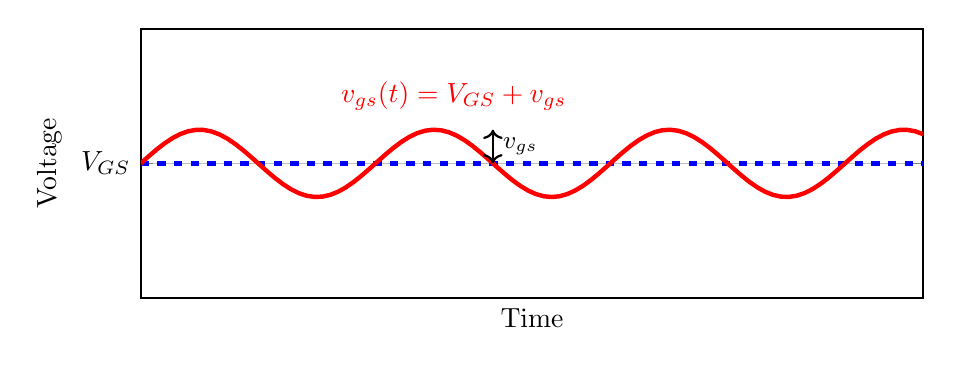
\begin{tikzpicture}
\begin{axis}[
    width=0.95\textwidth,
    height=5cm,
    xlabel={Time},
    ylabel={Voltage},
    xmin=0, xmax=10,
    ymin=0, ymax=4,
    xtick=\empty,
    ytick={2},
    yticklabels={$V_{GS}$},
    grid=major,
    thick,
]

% DC level
\addplot[blue, dashed, ultra thick, domain=0:10] {2};

% AC signal
\addplot[red, ultra thick, domain=0:10, samples=100] {2 + 0.5*sin(deg(2*pi*x/3))};
\node[red] at (axis cs:4,3) {$v_{gs}(t) = V_{GS} + v_{gs}$};

% Small signal annotation
\draw[<->] (axis cs:4.5,2) -- (axis cs:4.5,2.5);
\node[right, font=\small] at (axis cs:4.5,2.25) {$v_{gs}$};

\end{axis}
\end{tikzpicture}

\begin{block}{Key Concept}
AC analysis assumes small signals ($v_{gs} \ll V_{GS}$), allowing linear approximation around the Q-point.
\end{block}
\end{column}
\end{columns}
\end{frame}

% Slide 4: Small-Signal Concept
\begin{frame}{Small-Signal Linearization}
\begin{columns}
\begin{column}{0.5\textwidth}
\textbf{Nonlinear DC Relationship}
\[
i_D = k_n (v_{GS} - V_{th})^2 (1 + \lambda v_{DS})
\]

% \vspace{0.3cm}
\textbf{Total signals:}
\[
\begin{aligned}
v_{GS}(t) &= V_{GS} + v_{gs}(t) \\
v_{DS}(t) &= V_{DS} + v_{ds}(t) \\
i_D(t) &= I_D + i_d(t)
\end{aligned}
\]

% \vspace{0.3cm}
\textbf{Taylor Series Expansion}
\[
i_D(t) = I_D + \frac{\partial i_D}{\partial v_{GS}}\bigg|_Q v_{gs} + \frac{\partial i_D}{\partial v_{DS}}\bigg|_Q v_{ds} + \ldots
\]

% \vspace{0.3cm}
For small signals, higher-order terms negligible.
\end{column}

\begin{column}{0.5\textwidth}
\textbf{Graphical Interpretation}

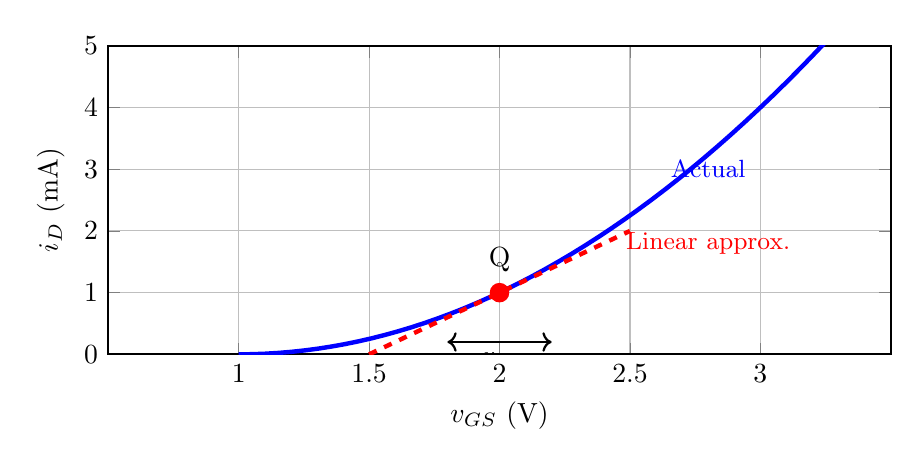
\begin{tikzpicture}
\begin{axis}[
    width=0.95\textwidth,
    height=5.5cm,
    xlabel={$v_{GS}$ (V)},
    ylabel={$i_D$ (mA)},
    xmin=0.5, xmax=3.5,
    ymin=0, ymax=5,
    xtick={1, 1.5, 2, 2.5, 3},
    ytick={0, 1, 2, 3, 4, 5},
    grid=major,
    thick,
]

% Nonlinear characteristic (saturation)
\addplot[blue, ultra thick, domain=1:3.5, samples=50] {(x-1)^2};

% Q-point
\node[circle, fill=red, inner sep=2.5pt, label=above:{Q}] at (axis cs:2,1) {};

% Tangent line (small-signal approximation)
\addplot[red, dashed, ultra thick, domain=1.5:2.5] {2*(x-2)+1};

% Small signal region
\draw[<->, thick] (axis cs:1.8,0.2) -- (axis cs:2.2,0.2);
\node[below, font=\small] at (axis cs:2,0.2) {$v_{gs}$};

\node[blue, font=\small] at (axis cs:2.8,3) {Actual};
\node[red, font=\small] at (axis cs:2.8,1.8) {Linear approx.};

\end{axis}
\end{tikzpicture}

\vspace{-0.1cm}
Slope at Q-point = transconductance $g_m$
\end{column}
\end{columns}
\end{frame}

% Slide 5: Voltage Gain from Transconductance
\begin{frame}{Common Source Amplifier: Voltage Gain Mechanism}
\begin{columns}[T]
\begin{column}{0.5\textwidth}
\textbf{Small Changes in $V_{GS}$ Create Large Changes in $V_{DS}$}

\vspace{0.15cm}

Consider a common source amplifier biased at Q-point:
\begin{itemize}
\item Input signal varies $v_{GS}$
\item This modulates drain current $i_D$
\item Current flows through load resistor $R_D$
\item Output voltage $v_{DS}$ changes
\end{itemize}


\begin{block}{Voltage Gain}
Small $\Delta v_{GS}$ $\Rightarrow$ Large $\Delta i_D$ $\Rightarrow$ Large $\Delta v_{DS}$

This is the fundamental amplification mechanism.
\end{block}

\end{column}

\begin{column}{0.5\textwidth}
\textbf{Voltage Transfer Characteristic (VTC)}

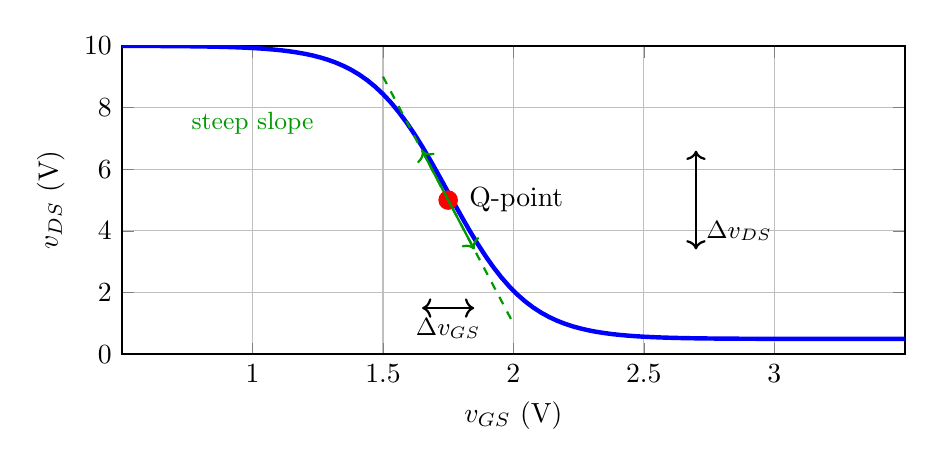
\begin{tikzpicture}
\begin{axis}[
    width=0.95\textwidth,
    height=5.5cm,
    xlabel={$v_{GS}$ (V)},
    ylabel={$v_{DS}$ (V)},
    xmin=0.5, xmax=3.5,
    ymin=0, ymax=10,
    xtick={1, 1.5, 2, 2.5, 3},
    ytick={0, 2, 4, 6, 8, 10},
    grid=major,
    thick,
]

% VTC curve
\addplot[blue, ultra thick, domain=0.5:3.5, samples=100] {9.5 / (1 + exp(6.5*(x - 1.75))) + 0.5};

% Q-point
\node[circle, fill=red, inner sep=2.5pt, label=right:{Q-point}] at (axis cs:1.75,5) {};

% Small signal variation
\draw[<->, thick, green!60!black] (axis cs:1.65,6.6) -- (axis cs:1.85,3.4);

% Input variation annotation
\draw[<->, thick] (axis cs:1.65,1.5) -- (axis cs:1.85,1.5);
\node[below, font=\small] at (axis cs:1.75,1.5) {$\Delta v_{GS}$};

% Output variation annotation
\draw[<->, thick] (axis cs:2.7,3.4) -- (axis cs:2.7,6.6);
\node[right, font=\small] at (axis cs:2.7,4) {$\Delta v_{DS}$ };

% Slope annotation 
\draw[green!60!black, thick, dashed, domain=1.5:2.0] (axis cs:1.5,9) -- (axis cs:2.0,1);
\node[green!60!black, font=\small] at (axis cs:1,7.5) {steep slope};

\end{axis}
\end{tikzpicture}

\vspace{-0.5cm}

\textbf{Voltage Gain:}
\[
A_v = \frac{\Delta v_{DS}}{\Delta v_{GS}} = \text{slope of VTC}
\]

The steeper the slope, the higher the gain!
\end{column}
\end{columns}
\end{frame}

% Slide 6: Transconductance (gm)
\begin{frame}{Transconductance $g_m$}
\begin{columns}
\begin{column}{0.5\textwidth}
\textbf{Definition}

Transconductance relates small-signal gate voltage to drain current:
\[
g_m = \frac{\partial i_D}{\partial v_{GS}}\bigg|_Q
\]

\vspace{-0.2cm}
\textbf{Derivation (Saturation, no CLM)}
\[
I_D = k_n (V_{GS} - V_{th})^2
\]
\[
g_m = \frac{\partial}{\partial V_{GS}} \left[ k_n (V_{GS} - V_{th})^2 \right]
\]
\[
\boxed{g_m = 2 k_n (V_{GS} - V_{th}) = 2 k_n V_{OV}}
\]

where $V_{OV} = V_{GS} - V_{th}$, overdrive voltage.
\end{column}

\begin{column}{0.5\textwidth}
\textbf{Alternative Forms}

Since $I_D = k_n V_{OV}^2$, we can write:
\[
\boxed{g_m = \sqrt{2 k_n I_D} = \frac{2 I_D}{V_{OV}}}
\]

% \vspace{0.3cm}
\textbf{Units:} mA/V or mS (millisiemens)

% \vspace{0.5cm}
\textbf{Physical Interpretation}
\begin{itemize}
\item[\gooditem] Voltage-to-current gain
\item[\gooditem] Larger $g_m$ = better amplification
\item[\gooditem] Increases with $I_D$ and device size ($W/L$)
\item[\baditem] Decreases with $V_{OV}$ (for fixed $I_D$)
\end{itemize}

% \vspace{0.3cm}
\begin{block}{Important}
$g_m$ is determined by the DC operating point
\end{block}
\end{column}
\end{columns}
\end{frame}

% Slide 6: Output Resistance (ro)
\begin{frame}{Output Resistance $r_o$ - Channel Length Modulation}
\begin{columns}
\begin{column}{0.5\textwidth}
\textbf{Channel-Length Modulation (CLM)}

In saturation, $I_D$ depends slightly on $V_{DS}$:
\[
I_D = k_n (V_{GS} - V_{th})^2 (1 + \lambda V_{DS})
\]

where $\lambda$ is the CLM parameter (V$^{-1}$).

\textbf{Output Resistance}
\[
r_o = \frac{\partial v_{DS}}{\partial i_D}\bigg|_Q 
\]

\vspace{-0.2cm}

\textbf{Derivation:}
\[
\frac{\partial i_D}{\partial v_{DS}} = k_n (V_{GS} - V_{th})^2 \lambda = \lambda I_D
\]
\[
\boxed{r_o = \frac{1}{\lambda I_D}}
\]
\end{column}

\begin{column}{0.5\textwidth}
\textbf{I-V Curves with CLM}

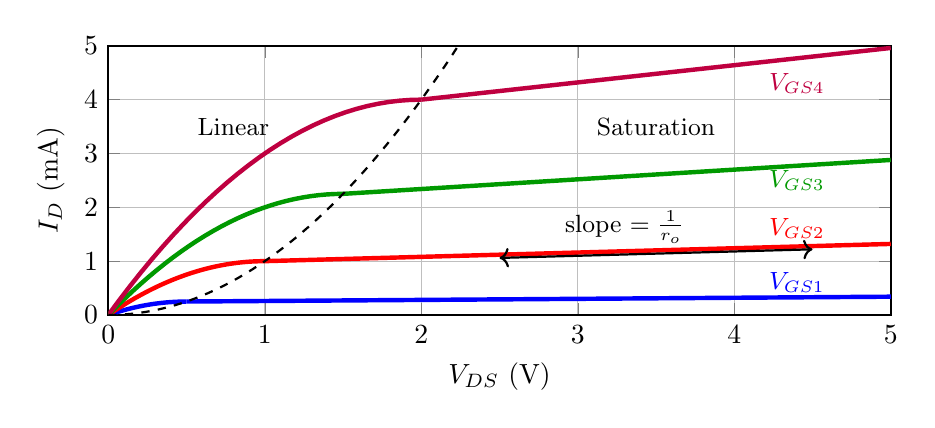
\begin{tikzpicture}
\begin{axis}[
    width=0.95\textwidth,
    height=5cm,
    xlabel={$V_{DS}$ (V)},
    ylabel={$I_D$ (mA)},
    xmin=0, xmax=5,
    ymin=0, ymax=5,
    xtick={0, 1, 2, 3, 4, 5},
    ytick={0, 1, 2, 3, 4, 5},
    grid=major,
    thick,
]

% VGS = 1.0V (V_OV = 0.5V)
\addplot[blue, ultra thick, domain=0:0.5, samples=30] {x - x^2};
\addplot[blue, ultra thick, domain=0.5:5, samples=30] {0.25*(1+0.08*(x-0.5))};

% VGS = 1.5V (V_OV = 1.0V)
\addplot[red, ultra thick, domain=0:1.0, samples=30] {2*x - x^2};
\addplot[red, ultra thick, domain=1.0:5, samples=30] {1.0*(1+0.08*(x-1.0))};

% VGS = 2.0V (V_OV = 1.5V)
\addplot[green!60!black, ultra thick, domain=0:1.5, samples=30] {3*x - x^2};
\addplot[green!60!black, ultra thick, domain=1.5:5, samples=30] {2.25*(1+0.08*(x-1.5))};

% VGS = 2.5V (V_OV = 2.0V)
\addplot[purple, ultra thick, domain=0:2.0, samples=30] {4*x - x^2};
\addplot[purple, ultra thick, domain=2.0:5, samples=30] {4.0*(1+0.08*(x-2.0))};

% Saturation boundary (parabola)
\addplot[black, dashed, thick, domain=0:2.236, samples=50] {x^2};

% Slope annotation in saturation region
\draw[<->, thick, black] (axis cs:2.5,1.06) -- (axis cs:4.5,1.22);
\node[above, font=\small, black] at (axis cs:3.3,1.14) {slope $= \frac{1}{r_o}$};

% Region labels
\node[font=\small] at (axis cs:0.8,3.5) {Linear};
\node[font=\small] at (axis cs:3.5,3.5) {Saturation};

% VGS labels
\node[font=\small, blue] at (axis cs:4.4,0.6) {$V_{GS1}$};
\node[font=\small, red] at (axis cs:4.4,1.6) {$V_{GS2}$};
\node[font=\small, green!60!black] at (axis cs:4.4,2.5) {$V_{GS3}$};
\node[font=\small, purple] at (axis cs:4.4,4.3) {$V_{GS4}$};

\end{axis}
\end{tikzpicture}

\vspace{-0.3cm}
\textbf{Typical Values}
\begin{itemize}
\item $\lambda = 0.01$ to $0.1$ V$^{-1}$
\item $r_o = 10$ to $100$ k$\Omega$
\item[\gooditem] Higher $r_o$ = better current source
\end{itemize}
\end{column}
\end{columns}
\end{frame}

% Slide 7: Small-Signal Model
\begin{frame}{MOSFET Small-Signal Equivalent Circuit}
\begin{columns}[T]
\begin{column}{0.5\textwidth}
\textbf{Small-Signal Model (Saturation)}

% \vspace{0.3cm}

\begin{circuitikz}[scale=0.8, transform shape]
% Gate terminal 
\draw (0,2.5) node[left] {G} to[short, o-] (0.8,2.5);

% Source terminal 
\draw (0,0.5) node[left] {S} to[short, o-] (0.8,0.5);
\draw (0.8,0.5) to[short] (4.5,0.5);

% Drain terminal
\draw (0,4.5) node[left] {D} to[short, o-] (2.5,4.5);

% Controlled current source 
\draw (2.5,4.5) to[american current source, l=$g_m v_{gs}$] (2.5,0.5);

% Output resistance in parallel
\draw (2.5,4.5) to[short] (4.5,4.5);
\draw (4.5,4.5) to[R, l=$r_o$] (4.5,0.5);

% v_gs voltage 
\node[font=\small] at (0.8,2.1) {$+$};
\node[font=\small] at (0.8,1.5) {$v_{gs}$};
\node[font=\small] at (0.8,0.8) {$-$};

% v_ds voltage 
\node[font=\small] at (1.2,4.1) {$+$};
\node[font=\small] at (1.2,2.5) {$v_{ds}$};
\node[font=\small] at (1.2,0.8) {$-$};

% Current label 
\draw[->, >=latex, thick, blue] (1.5,4.5) -- (2.2,4.5);
\node[above, blue, font=\small] at (1.85,4.5) {$i_d$};

\end{circuitikz}

% \vspace{-0.2cm}
\textbf{Key Features:}
\begin{itemize}
\item Voltage-controlled current source
\item Infinite input resistance (DC/low freq)
\item Finite output resistance $r_o$
\end{itemize}
\end{column}

\begin{column}{0.5\textwidth}
\textbf{Small-Signal Parameters}

\begin{table}[]
\begin{tabular}{|l|l|}
\hline
\textbf{Parameter} & \textbf{Expression} \\ \hline
$g_m$ & $2k_n V_{OV} = \sqrt{2k_n I_D}$ \\ \hline
$r_o$ & $\frac{1}{\lambda I_D}$ \\ \hline
$i_d$ & $g_m v_{gs} + \frac{v_{ds}}{r_o}$ \\ \hline
\end{tabular}
\end{table}

\textbf{Simplified Model ($r_o \to \infty$ / $\lambda = 0$)}

\vspace{-0.1cm}

\[
\boxed{i_d = g_m v_{gs}}
\]

\vspace{-0.2cm}

\begin{block}{The small-signal model is only valid for:}
\begin{itemize}
\item Small signal amplitudes
\item Frequencies where capacitances can be ignored
\item Operation in saturation region
\end{itemize}
\end{block}
\end{column}
\end{columns}
\end{frame}

% Slide 8: Example - Calculate Small-Signal Parameters
\begin{frame}{Example: Small-Signal Parameter Calculation}
\begin{columns}[T]
\begin{column}{0.45\textwidth}
\textbf{Given DC Operating Point:}
\begin{itemize}
\item $V_{GS} = 2$ V
\item $V_{DS} = 6$ V
\item $I_D = 2$ mA
\item $V_{th} = 1$ V
\item $k_n = 2$ mA/V$^2$
\item $\lambda = 0.02$ V$^{-1}$
\end{itemize}

\vspace{0.3cm}
\textbf{Find:} $g_m$ and $r_o$

\vspace{0.3cm}
\textbf{Solution:}

\textbf{Step 1:} Calculate overdrive voltage
\[
V_{OV} = V_{GS} - V_{th} = 2 - 1 = 1 \text{ V}
\]
\end{column}

\begin{column}{0.55\textwidth}
\textbf{Step 2:} Calculate transconductance

Using $g_m = 2k_n V_{OV}$:
\[
g_m = 2 \times 2 \times 1 = 4 \text{ mA/V}
\]

% \vspace{0.3cm}
\textbf{Step 3:} Calculate output impedance
\[
r_o = \frac{1}{\lambda I_D} = \frac{1}{0.02 \times 2 \times 10^{-3}} = \frac{1}{4 \times 10^{-5}}
\]
\[
\boxed{r_o = 25 \text{ k}\Omega}
\]

\vspace{0.3cm}
\textbf{Result:} Small-signal model has $g_m = 4$ mA/V and $r_o = 25$ k$\Omega$.
\end{column}
\end{columns}
\end{frame}

% Slide 9: AC Analysis Procedure
\begin{frame}{AC Analysis Procedure}
\begin{columns}[T]
\begin{column}{0.48\textwidth}
\begin{enumerate}
\item \textbf{Perform DC Analysis}
   \begin{itemize}
   \item Find Q-point: $V_{GS}$, $V_{DS}$, $I_D$
   \item Verify operating region
   \end{itemize}

\vspace{0.3cm}
\item \textbf{Calculate Small-Signal Parameters}
   \begin{itemize}
   \item $g_m = 2k_n V_{OV}$ or $g_m = \sqrt{2k_n I_D}$
   \item $r_o = \frac{1}{\lambda I_D}$ (if CLM included)
   \end{itemize}

\vspace{0.3cm}
\item \textbf{Draw AC Equivalent Circuit}
   \begin{itemize}
   \item Replace MOSFET with small-signal model
   \item DC sources $\to$ ground (short circuit)
   \item Capacitors $\to$ short circuit (at high frequencies)
   \item DC biasing resistors remain
   \end{itemize}
\end{enumerate}
\end{column}

\begin{column}{0.48\textwidth}
\begin{enumerate}
\setcounter{enumi}{3}
\item \textbf{Analyze AC Circuit}
   \begin{itemize}
   \item Apply KVL, KCL, Ohm's law
   \item Calculate voltage gain, input/output impedance
   \end{itemize}
\end{enumerate}

\vspace{0.5cm}

\begin{block}{Key Point}
Always perform DC analysis first to establish the Q-point before conducting AC analysis.
\end{block}
\end{column}
\end{columns}
\end{frame}

% Slide 10: Simple AC Example - Common Source Amplifier
\begin{frame}{Example: Common Source Amplifier Analysis}
\begin{columns}[T]
\begin{column}{0.35\textwidth}
\textbf{DC Circuit}

\vspace{0.2cm}

\begin{circuitikz}[scale=0.65, transform shape]
% VDD
\draw (0,5) to[short, o-] (0,4.5) node[above] at (0,5) {$V_{DD}$};
% RD
\draw (0,4.5) to[R, l=$R_D$] (0,2.5);
% MOSFET
\draw (0,2.5) node[nmos, arrowmos, anchor=drain] (M1) {};
\draw (M1.source) to[short] (0,0) node[ground] {};
% Gate bias
\draw (-2,1.7) to[short, o-] (-2,1.75) node[above] {$V_{GG}$};
\draw (-2,1.7) to[short] (M1.gate);
% Output
\draw (0,2.5) to[short, -o] (1,2.5) node[right] {$v_o$};
% Input
\draw (-3,1.7) to[sV, l=$v_{in}$] (-3,0) node[ground] {};
\draw (-3,1.7) to[C, l=$C_c$] (-2,1.7);
\end{circuitikz}

\vspace{0.3cm}
\textbf{Given:}
\begin{itemize}
\item $R_D = 2$ k$\Omega$
\item $g_m = 4$ mA/V
\item $r_o = 25$ k$\Omega$
\end{itemize}
\end{column}

\begin{column}{0.65\textwidth}
\textbf{AC Equivalent Circuit}

\vspace{0.2cm}

\begin{circuitikz}[scale=0.8, transform shape]
% Input voltage source
\draw (1,2) to[sV, l=$v_{in}$] (1,0) node[ground] {};
\draw (1,2) to[short, -o] (2.5,2);

% Gate terminal (open circuit - no connection to anything else)
\node[right, font=\small] at (2.5,2) {G};

% Source terminal at ground
\draw (3.5,0) node[ground] {} to[short] (8.5,0);
\node[above, font=\small] at (3.5,0.2) {S};

% Controlled current source (gmvgs) from drain to source
\draw (4.5,4.5) to[american current source, l=$g_m v_{gs}$] (4.5,0);

% Output resistance from drain to source
\draw (6.5,4.5) to[R, l=$r_o$] (6.5,0);

% RD from drain to ground (AC ground)
\draw (4.5,4.5) to[short] (6.5,4.5);
\draw (6.5,4.5) to[short] (8,4.5);
\draw (8,4.5) to[R, l=$R_D$] (8,0);

% Drain terminal and output
\draw (4.5,4.5) to[short, -o] (4.5,5);
\node[above, font=\small] at (4.5,5) {D};
\draw (6.5,4.5) to[short, -o] (9,4.5) node[right] {$v_{out}$};

% v_gs voltage 
\node[font=\small] at (2.75,1.8) {$+$};
\node[font=\small] at (2.75,1) {$v_{gs}$};
\node[font=\small] at (2.75,0.3) {$-$};

\end{circuitikz}

\vspace{0.3cm}
\textbf{Analysis:}

$v_{gs} = v_{in}$ (ideal coupling)

\vspace{0.2cm}
Current through $R_D$ and $r_o$ in parallel:
\[
i_d = g_m v_{gs} = g_m v_{in}
\]

Output voltage:
\[
v_{out} = -i_d (R_D \parallel r_o) = -g_m v_{in} (R_D \parallel r_o)
\]

Voltage gain:
\[
A_v = \frac{v_{out}}{v_{in}} = -g_m (R_D \parallel r_o)
\]
\[
A_v = -4 \times (2 \parallel 25) = -4 \times 1.85 = \boxed{-7.4}
\]
\end{column}
\end{columns}
\end{frame}

% Slide 11: Small-Signal Analysis
\begin{frame}{Example: Common Source Amplifier - Small-Signal Analysis}
\begin{columns}[T]
\begin{column}{0.5\textwidth}

\begin{circuitikz}[scale=0.7, transform shape]
% Input voltage source
\draw (1,2) to[sV, l=$v_{in}$] (1,0) node[ground] {};
\draw (1,2) to[short, -o] (2.5,2);

% Gate terminal (open circuit - no connection to anything else)
\node[right, font=\small] at (2.5,2) {G};

% Source terminal at ground
\draw (3.5,0) node[ground] {} to[short] (8.5,0);
\node[above, font=\small] at (3.5,0.2) {S};

% Controlled current source (gmvgs) from drain to source
\draw (4.5,4.5) to[american current source, l=$g_m v_{gs}$] (4.5,0);

% Output resistance from drain to source
\draw (6.5,4.5) to[R, l=$r_o$] (6.5,0);

% RD from drain to ground (AC ground)
\draw (4.5,4.5) to[short] (6.5,4.5);
\draw (6.5,4.5) to[short] (8,4.5);
\draw (8,4.5) to[R, l=$R_D$] (8,0);

% Drain terminal and output
\draw (4.5,4.5) to[short, -o] (4.5,5);
\node[above, font=\small] at (4.5,5) {D};
\draw (6.5,4.5) to[short, -o] (9,4.5) node[right] {$v_{out}$};

% v_gs voltage 
\node[font=\small] at (2.75,1.8) {$+$};
\node[font=\small] at (2.75,1) {$v_{gs}$};
\node[font=\small] at (2.75,0.3) {$-$};

\end{circuitikz}

\textbf{Given:}
\begin{itemize}
\item $R_D = 2$ k$\Omega$
\item $g_m = 4$ mA/V
\item $r_o = 25$ k$\Omega$
\end{itemize}
\end{column}

\begin{column}{0.5\textwidth}
\textbf{Small-Signal Analysis:}

\textbf{Current $i_d$} from controlled source
\[
i_d = g_m v_{gs} = g_m v_{in}
\]
\textbf{Output voltage}  (KVL at drain node)
Current flows through $R_D \parallel r_o$:
\[
v_{out} = -i_d (R_D \parallel r_o) = -g_m v_{in} (R_D \parallel r_o)
\]
\[
A_v = \frac{v_{out}}{v_{in}} = -g_m (R_D \parallel r_o)
\]
\[
R_D \parallel r_o = \frac{2 \times 25}{2 + 25} = 1.85 \text{ k}\Omega
\]
\[
A_v = -4 \times 1.85 = -7.4
\]
\end{column}
\end{columns}
\end{frame}

% Slide 12: Effect of ro on Gain
\begin{frame}{Impact of Output Resistance on Gain}
\begin{columns}[T]
\begin{column}{0.5\textwidth}
\textbf{Voltage Gain with CLM}
\[
A_v = -g_m (R_D \parallel r_o) = -g_m \frac{R_D r_o}{R_D + r_o}
\]

\textbf{Two Limiting Cases:}

\textbf{Case 1:} $r_o \gg R_D$ (ideal case)
\[
A_v \approx -g_m R_D
\]
Maximum achievable gain.

\textbf{Case 2:} $r_o \ll R_D$ (high CLM)
\[
A_v \approx -g_m r_o = -\frac{g_m}{\lambda I_D}
\]
Gain limited by device physics.
\end{column}

\begin{column}{0.5\textwidth}
\textbf{Gain vs. $r_o$}

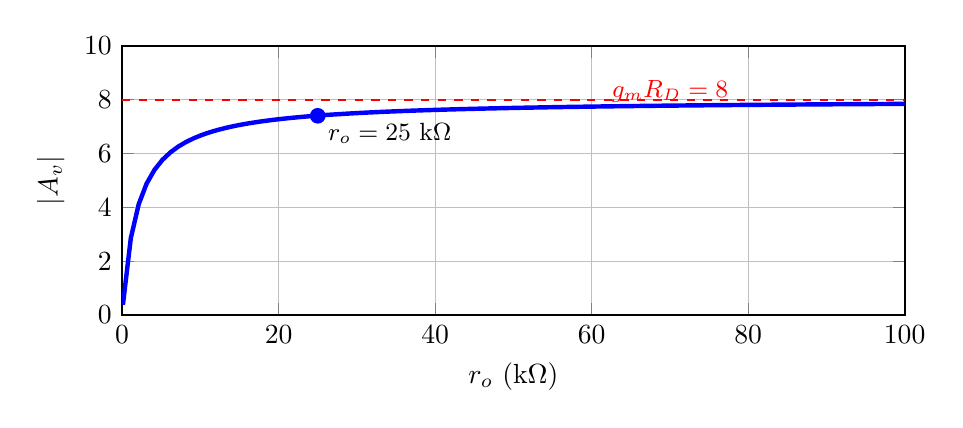
\begin{tikzpicture}
\begin{axis}[
    width=0.95\textwidth,
    height=5cm,
    xlabel={$r_o$ (k$\Omega$)},
    ylabel={$|A_v|$},
    xmin=0, xmax=100,
    ymin=0, ymax=10,
    xtick={0, 20, 40, 60, 80, 100},
    ytick={0, 2, 4, 6, 8, 10},
    grid=major,
    thick,
]

% Gain curve: |Av| = gm * (RD || ro), with gm=4, RD=2k
\addplot[blue, ultra thick, domain=0.1:100, samples=100] {4 * (2*x)/(2+x)};

% Asymptote
\addplot[red, dashed, thick, domain=0:100] {8};
\node[red, font=\small] at (axis cs:70,8.3) {$g_m R_D = 8$};

% Example point
\node[circle, fill=blue, inner sep=2pt] at (axis cs:25,7.4) {};
\node[above right, font=\small] at (axis cs:25,6) {$r_o = 25$ k$\Omega$};

\end{axis}
\end{tikzpicture}

\vspace{-0.3cm}
\textbf{Design Insight:}
\begin{itemize}
\item[\gooditem] Higher $r_o$ improves gain
\item[\gooditem] Long-channel devices have higher $r_o$
\end{itemize}
\end{column}
\end{columns}
\end{frame}

% Slide 13: Summary of Small-Signal Parameters
\begin{frame}{Summary: MOSFET Small-Signal Parameters}
\begin{table}[]
\centering
\begin{tabular}{|l|l|l|l|}
\hline
\textbf{Parameter} & \textbf{Definition} & \textbf{Formula} & \textbf{Typical Value} \\ \hline
Transconductance & $\frac{\partial i_D}{\partial v_{GS}}$ & $g_m = 2k_n V_{OV} = \sqrt{2k_n I_D}$ & 1-10 mA/V \\ \hline
Output resistance & $\frac{\partial v_{DS}}{\partial i_D}$ & $r_o = \frac{1}{\lambda I_D}$ & 10-100 k$\Omega$ \\ \hline
Body transconductance & $\frac{\partial i_D}{\partial v_{BS}}$ & $g_{mb} = \eta g_m$ & 0.1-0.3 $g_m$ \\ \hline
\end{tabular}
\end{table}

\vspace{0.5cm}

\begin{columns}
\begin{column}{0.5\textwidth}
\textbf{Key Relationships:}
\begin{itemize}
\item $g_m \propto \sqrt{I_D}$
\item $g_m \propto \sqrt{W/L}$
\item $r_o \propto 1/I_D$
\item $g_m \cdot r_o = \frac{2}{\lambda V_{OV}}$ (intrinsic gain)
\end{itemize}
\end{column}

\begin{column}{0.5\textwidth}
\textbf{Design Trade-offs:}
\begin{itemize}
\item Large $I_D$ $\Rightarrow$ high $g_m$, low $r_o$
\item Large $W/L$ $\Rightarrow$ high $g_m$, more area
\item Small $V_{OV}$ $\Rightarrow$ high $g_m$ (for given $I_D$)
\item Long channel $\Rightarrow$ small $\lambda$, high $r_o$
\end{itemize}
\end{column}
\end{columns}
\end{frame}

\end{document}
